\documentclass[12pt,a4paper]{article}

\usepackage[a4paper,margin=0.75in]{geometry}
\usepackage[T1]{fontenc}
\usepackage[utf8]{inputenc}
\usepackage{xcolor}
\usepackage{tikz}
\usepackage{float}
\usepackage{caption}
\usetikzlibrary{arrows.meta, positioning, shadows, fit, backgrounds, calc}

\DeclareRobustCommand{\code}[1]{\texttt{\detokenize{#1}}}
\captionsetup{font=small,labelfont=bf}
\setlength{\emergencystretch}{4em}

\definecolor{dialogueFill}{RGB}{232,242,255}
\definecolor{groundFill}{RGB}{255,245,230}
\definecolor{plannerFill}{RGB}{235,249,240}
\definecolor{execFill}{RGB}{245,232,255}
\definecolor{skillFill}{RGB}{244,244,244}
\definecolor{busFill}{RGB}{232,235,240}
\definecolor{futureFill}{RGB}{255,240,240}
\definecolor{ink}{RGB}{40,50,65}
\definecolor{blueLine}{RGB}{37,67,105}
\definecolor{greenLine}{RGB}{184,100,24}
\definecolor{orangeLine}{RGB}{146,89,34}
\definecolor{purpleLine}{RGB}{92,63,139}
\definecolor{grayLine}{RGB}{115,122,135}

\tikzset{
  nodebox/.style={
    draw=ink!70,
    thick,
    rounded corners=2pt,
    align=center,
    minimum height=9mm,
    inner xsep=5pt,
    inner ysep=4pt,
    font=\scriptsize,
    fill=white,
    drop shadow={shadow xshift=.45pt, shadow yshift=-.45pt, opacity=.12}
  },
  lane/.style={
    draw=grayLine!60,
    thick,
    rounded corners=5pt,
    inner sep=7pt,
    fill=white
  },
  input/.style={nodebox, fill=white},
  dialogueNode/.style={nodebox, fill=dialogueFill},
  groundNode/.style={nodebox, fill=groundFill},
  plannerNode/.style={nodebox, fill=plannerFill},
  execNode/.style={nodebox, fill=execFill},
  skillNode/.style={nodebox, fill=skillFill},
  futureNode/.style={nodebox, dashed, fill=futureFill},
  bus/.style={
    draw=grayLine!80,
    thick,
    rounded corners=3pt,
    fill=busFill,
    align=center,
    font=\scriptsize,
    inner ysep=3.5pt,
    inner xsep=5pt
  },
  control/.style={-{Latex[length=2.4mm,width=1.5mm]}, very thick, draw=blueLine},
  evidence/.style={-{Latex[length=2.2mm,width=1.4mm]}, thick, draw=greenLine},
  feedback/.style={-{Latex[length=2.2mm,width=1.4mm]}, thick, dashed, draw=orangeLine},
  adapter/.style={-{Latex[length=2.2mm,width=1.4mm]}, thick, draw=purpleLine},
  future/.style={-{Latex[length=2.0mm,width=1.2mm]}, thick, dashed, draw=grayLine},
  label/.style={font=\tiny, fill=white, inner sep=1pt}
}

\begin{document}

% ---------------------------------------------------------------------------
% Node diagram 1: chatbot_llm.
% ---------------------------------------------------------------------------
\begin{figure}[H]
\centering
\resizebox{\linewidth}{!}{%
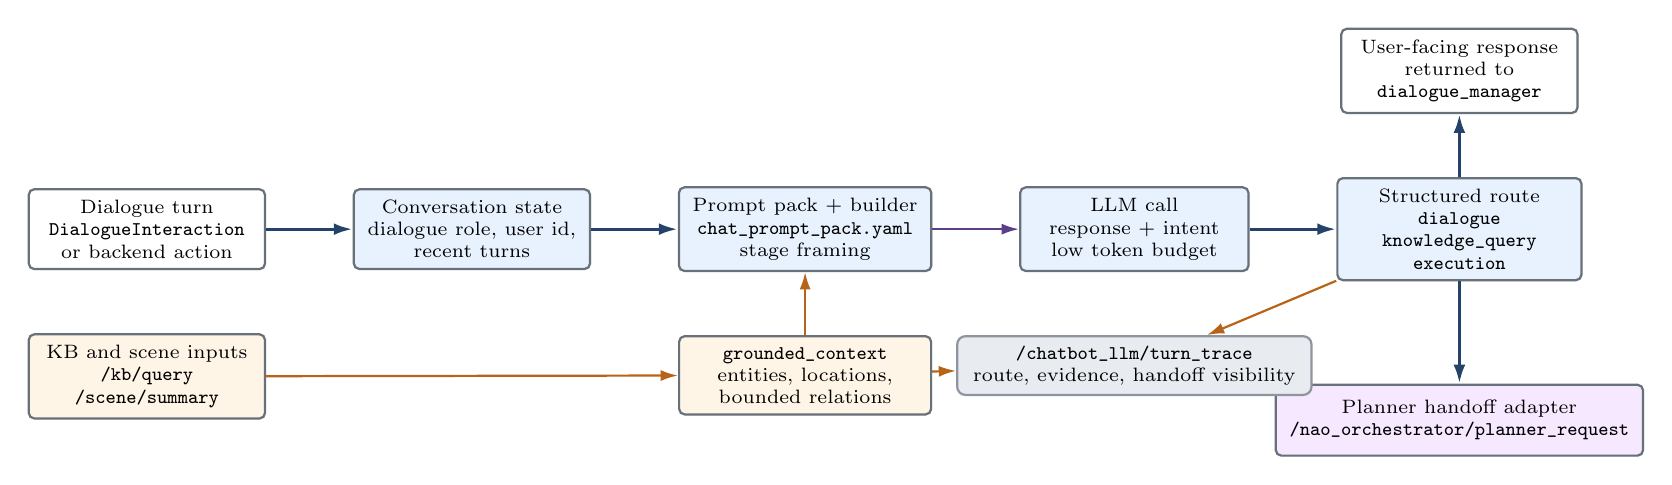
\begin{tikzpicture}[node distance=8mm and 11mm]
  \node[input, minimum width=30mm] (turn) {Dialogue turn\\\code{DialogueInteraction}\\or backend action};
  \node[groundNode, below=of turn, minimum width=30mm] (kb) {KB and scene inputs\\\code{/kb/query}\\\code{/scene/summary}};

  \node[dialogueNode, right=of turn, minimum width=30mm] (history) {Conversation state\\dialogue role, user id,\\recent turns};
  \node[dialogueNode, right=of history, minimum width=31mm] (prompt) {Prompt pack + builder\\\code{chat_prompt_pack.yaml}\\stage framing};
  \node[dialogueNode, right=of prompt, minimum width=29mm] (model) {LLM call\\response + intent\\low token budget};
  \node[dialogueNode, right=of model, minimum width=31mm] (route) {Structured route\\\code{dialogue}\\\code{knowledge_query}\\\code{execution}};

  \node[groundNode, below=of prompt, minimum width=32mm] (context) {\code{grounded_context}\\entities, locations,\\bounded relations};
  \node[execNode, below=13mm of route, minimum width=35mm] (handoff) {Planner handoff adapter\\\code{/nao_orchestrator/planner_request}};
  \node[input, above=of route, minimum width=30mm] (speech) {User-facing response\\returned to\\\code{dialogue_manager}};
  \node[bus, below=of model, minimum width=45mm] (trace) {\code{/chatbot_llm/turn_trace}\\route, evidence, handoff visibility};

  \draw[control] (turn) -- (history);
  \draw[evidence] (kb) -- (context);
  \draw[evidence] (context) -- (prompt);
  \draw[control] (history) -- (prompt);
  \draw[adapter] (prompt) -- (model);
  \draw[control] (model) -- (route);
  \draw[control] (route) -- (speech);
  \draw[control] (route) -- (handoff);
  \draw[evidence] (route) -- (trace);
  \draw[evidence] (context) -- (trace);
\end{tikzpicture}%
}
\caption{\code{chatbot_llm} node-level view. The node owns semantic turn interpretation and planner ingress metadata, but it does not create executable plans or dispatch robot skills.}
\label{fig:chatbot-llm-node}
\end{figure}

% ---------------------------------------------------------------------------
% Node diagram 2: planner_llm.
% ---------------------------------------------------------------------------
\begin{figure}[H]
\centering
\resizebox{\linewidth}{!}{%
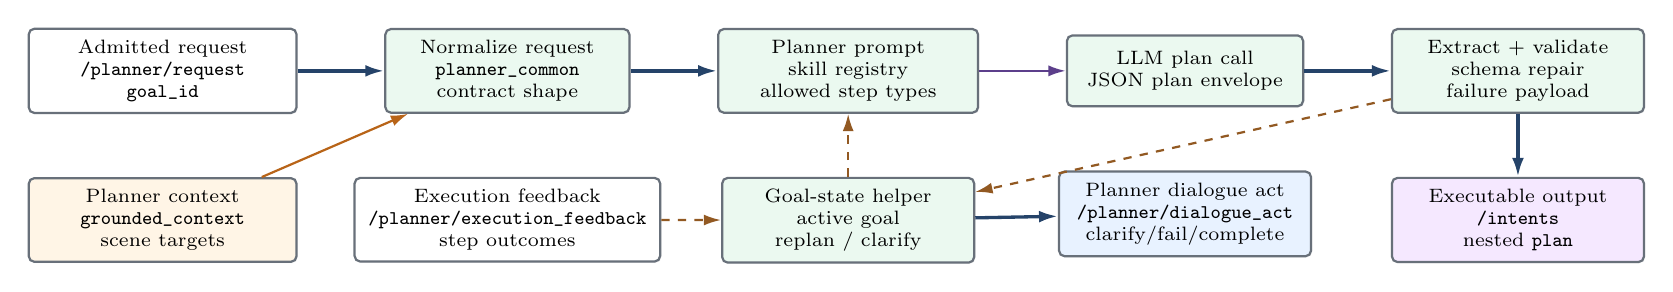
\begin{tikzpicture}[node distance=8mm and 11mm]
  \node[input, minimum width=34mm] (request) {Admitted request\\\code{/planner/request}\\\code{goal_id}};
  \node[groundNode, below=of request, minimum width=34mm] (ctx) {Planner context\\\code{grounded_context}\\scene targets};

  \node[plannerNode, right=of request, minimum width=31mm] (normalize) {Normalize request\\\code{planner_common}\\contract shape};
  \node[plannerNode, right=of normalize, minimum width=33mm] (prompt) {Planner prompt\\skill registry\\allowed step types};
  \node[plannerNode, right=of prompt, minimum width=30mm] (model) {LLM plan call\\JSON plan envelope};
  \node[plannerNode, right=of model, minimum width=32mm] (validate) {Extract + validate\\schema repair\\failure payload};

  \node[execNode, below=of validate, minimum width=32mm] (intent) {Executable output\\\code{/intents}\\nested \code{plan}};
  \node[plannerNode, below=of prompt, minimum width=32mm] (supervisor) {Goal-state helper\\active goal\\replan / clarify};
  \node[input, below=of normalize, minimum width=34mm] (feedback) {Execution feedback\\\code{/planner/execution_feedback}\\step outcomes};
  \node[dialogueNode, below=of model, minimum width=32mm] (act) {Planner dialogue act\\\code{/planner/dialogue_act}\\clarify/fail/complete};

  \draw[control] (request) -- (normalize);
  \draw[evidence] (ctx) -- (normalize);
  \draw[control] (normalize) -- (prompt);
  \draw[adapter] (prompt) -- (model);
  \draw[control] (model) -- (validate);
  \draw[control] (validate) -- (intent);
  \draw[feedback] (feedback) -- (supervisor);
  \draw[feedback] (supervisor) -- (prompt);
  \draw[control] (supervisor) -- (act);
  \draw[feedback] (validate) -- (supervisor);
\end{tikzpicture}%
}
\caption{\code{planner_llm} node-level view. The planner generates structured plan envelopes and maintains feedback-driven goal state; execution and speech remain downstream responsibilities.}
\label{fig:planner-llm-node}
\end{figure}

% ---------------------------------------------------------------------------
% Node diagram 3: nao_orchestrator.
% ---------------------------------------------------------------------------
\begin{figure}[H]
\centering
\resizebox{\linewidth}{!}{%
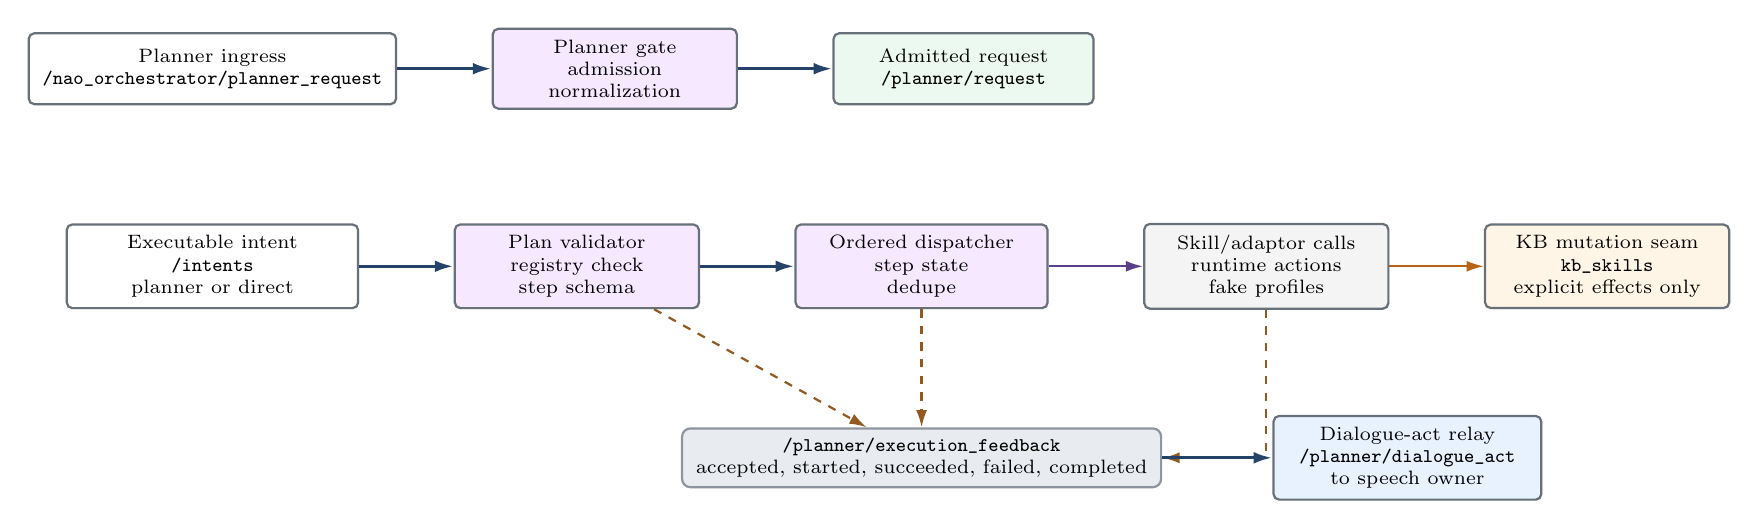
\begin{tikzpicture}[node distance=9mm and 12mm]
  \node[input, minimum width=37mm] (ingress) {Planner ingress\\\code{/nao_orchestrator/planner_request}};
  \node[execNode, right=of ingress, minimum width=31mm] (gate) {Planner gate\\admission\\normalization};
  \node[plannerNode, right=of gate, minimum width=33mm] (publishReq) {Admitted request\\\code{/planner/request}};

  \node[input, below=15mm of ingress, minimum width=37mm] (intent) {Executable intent\\\code{/intents}\\planner or direct};
  \node[execNode, right=of intent, minimum width=31mm] (validator) {Plan validator\\registry check\\step schema};
  \node[execNode, right=of validator, minimum width=32mm] (dispatcher) {Ordered dispatcher\\step state\\dedupe};
  \node[skillNode, right=of dispatcher, minimum width=31mm] (skills) {Skill/adaptor calls\\runtime actions\\fake profiles};
  \node[groundNode, right=of skills, minimum width=31mm] (kbmut) {KB mutation seam\\\code{kb_skills}\\explicit effects only};

  \node[bus, below=15mm of dispatcher, minimum width=58mm] (feedback) {\code{/planner/execution_feedback}\\accepted, started, succeeded, failed, completed};
  \node[dialogueNode, right=14mm of feedback, minimum width=34mm] (relay) {Dialogue-act relay\\\code{/planner/dialogue_act}\\to speech owner};

  \draw[control] (ingress) -- (gate);
  \draw[control] (gate) -- (publishReq);
  \draw[control] (intent) -- (validator);
  \draw[control] (validator) -- (dispatcher);
  \draw[adapter] (dispatcher) -- (skills);
  \draw[evidence] (skills) -- (kbmut);
  \draw[feedback] (validator) -- (feedback);
  \draw[feedback] (dispatcher) -- (feedback);
  \draw[feedback] (skills) |- (feedback);
  \draw[control] (feedback) -- (relay);
\end{tikzpicture}%
}
\caption{\code{nao_orchestrator} node-level view. The orchestrator is the deterministic boundary for admission, validation, dispatch, feedback, and explicit KB mutation routing. It does not plan or produce LLM dialogue policy.}
\label{fig:nao-orchestrator-node}
\end{figure}

% ---------------------------------------------------------------------------
% Node diagram 4: perception / grounding pipeline.
% ---------------------------------------------------------------------------
\begin{figure}[H]
\centering
\resizebox{\linewidth}{!}{%
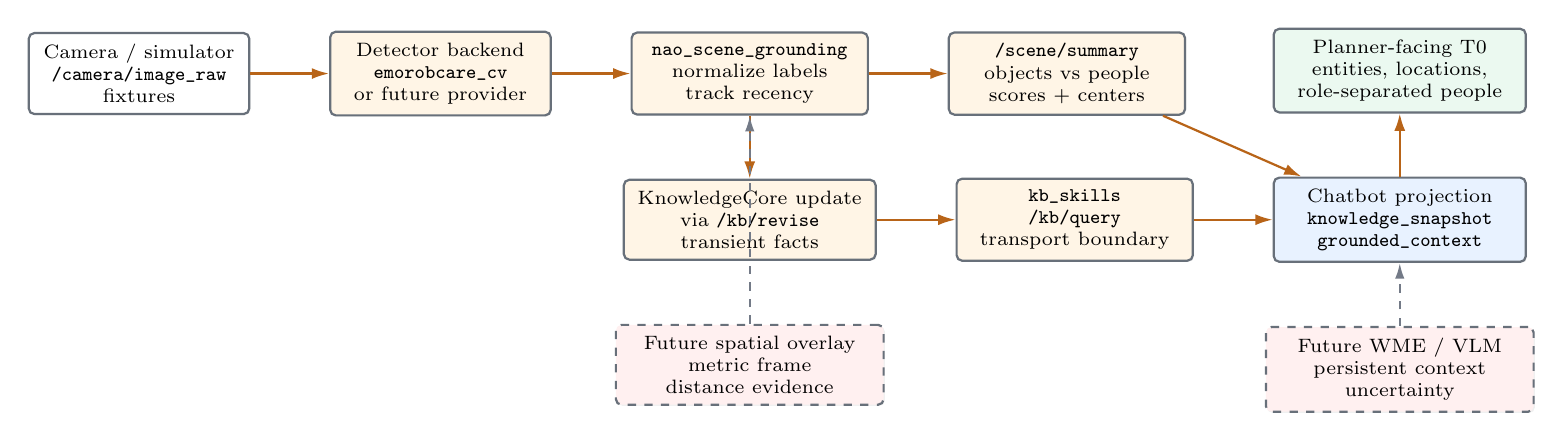
\begin{tikzpicture}[node distance=8mm and 10mm]
  \node[input, minimum width=28mm] (camera) {Camera / simulator\\\code{/camera/image_raw}\\fixtures};
  \node[groundNode, right=of camera, minimum width=28mm] (detector) {Detector backend\\\code{emorobcare_cv}\\or future provider};
  \node[groundNode, right=of detector, minimum width=30mm] (grounding) {\code{nao_scene_grounding}\\normalize labels\\track recency};
  \node[groundNode, right=of grounding, minimum width=30mm] (summary) {\code{/scene/summary}\\objects vs people\\scores + centers};

  \node[groundNode, below=of grounding, minimum width=30mm] (kb) {KnowledgeCore update\\via \code{/kb/revise}\\transient facts};
  \node[groundNode, right=of kb, minimum width=30mm] (kbskills) {\code{kb_skills}\\\code{/kb/query}\\transport boundary};
  \node[dialogueNode, right=of kbskills, minimum width=32mm] (projection) {Chatbot projection\\\code{knowledge_snapshot}\\\code{grounded_context}};

  \node[plannerNode, above=of projection, minimum width=32mm] (plannerContext) {Planner-facing T0\\entities, locations,\\role-separated people};
  \node[futureNode, below=of kb, minimum width=34mm] (overlay) {Future spatial overlay\\metric frame\\distance evidence};
  \node[futureNode, below=of projection, minimum width=34mm] (wme) {Future WME / VLM\\persistent context\\uncertainty};

  \draw[evidence] (camera) -- (detector);
  \draw[evidence] (detector) -- (grounding);
  \draw[evidence] (grounding) -- (summary);
  \draw[evidence] (grounding) -- (kb);
  \draw[evidence] (kb) -- (kbskills);
  \draw[evidence] (kbskills) -- (projection);
  \draw[evidence] (summary) -- (projection);
  \draw[evidence] (projection) -- (plannerContext);
  \draw[future] (overlay) -- (grounding);
  \draw[future] (wme) -- (projection);
\end{tikzpicture}%
}
\caption{Combined perception and grounding pipeline. Raw detector and KB evidence stays at its owning seams; chatbot and planner consume compact symbolic projections instead of raw perception streams.}
\label{fig:perception-grounding-pipeline}
\end{figure}

\end{document}
